\documentclass[sigconf, 10pt, anonymous, nonacm]{acmart}
\settopmatter{printfolios=true, printccs=false, printacmref=false}

\title{When Measurements Become Targets: The Strategic Manipulation Challenge for Internet Observatories}

\author{First Author}
\affiliation{%
  \institution{First Institution}
  \city{City}
  \country{Country}
}

\author{Second Author}
\affiliation{%
  \institution{Second Institution}
  \city{City}
  \country{Country}
}

\begin{abstract}
Internet observatories increasingly influence reputation, compliance assessments, and business relationships across the Internet ecosystem. Yet many of these observatories depend on measurement infrastructures that are public, long-lived, and therefore potentially recognizable to the networks they evaluate. As favorable measurement outcomes become increasingly valuable, operators may have incentives to optimize specifically for measurement platforms while behaving differently toward ordinary users and traffic. We refer to this phenomenon as \emph{measurement awareness} and argue that it represents an emerging challenge for Internet measurement.

Using Route Origin Validation (ROV) as a case study, we compare observations obtained using publicly known RPKI-invalid targets with those obtained using functionally equivalent but undisclosed shadow targets. We identify networks exhibiting behavior consistent with measurement awareness, rejecting well-known invalid prefixes while continuing to accept equivalent shadow prefixes. Our findings suggest that Internet observatories may not always capture the properties they intend to measure, but rather the behavior networks choose to expose to the measurement infrastructure.
\end{abstract}

\begin{document}

\maketitle

\section{Introduction}

Internet measurement plays a central role in understanding the operational state of the network~\cite{clark}. Researchers, operators, regulators, and policymakers rely on measurement studies to evaluate properties ranging from performance and reliability~\cite{zoom,mlab} to routing security~\cite{isbgpsafeyet,rscope,rovista} and censorship~\cite{CenRL, iris,censoredplanet}. Many of these studies rely on long-lived Internet observatories and shared measurement infrastructures that provide continuous visibility into network behavior.

A common challenge across these efforts is obtaining measurement vantage points that are sufficiently diverse, accessible, and reproducible. Geographic coverage, topological diversity, and experimental control are all desirable properties, yet satisfying them simultaneously is difficult in practice. As a result, a substantial fraction of Internet measurement research depends on a relatively small collection of shared, public, and long-lived infrastructures and observatories.

Although side-channel techniques~\cite{ipid,ipv6} can sometimes extend visibility beyond dedicated measurement infrastructures, they often provide limited experimental control and may disappear as implementations evolve~\cite{rscope}. In contrast, many measurement studies require stable platforms that remain comparable over long periods of time, making continuity and reproducibility valuable properties of Internet observatories.

The influence of these observatories increasingly extends beyond academic research. Measurements are routinely incorporated into security assessments, compliance initiatives, operational decisions, and commercial relationships. Consequently, favorable measurement outcomes can carry reputational and economic value for the networks being evaluated.

This evolution introduces an implicit assumption: that networks behave consistently regardless of who is observing them. In most studies, measurements are interpreted as reflecting the actual policies deployed by the network under observation rather than policies selectively exposed to the measurement process itself.

However, the characteristics that make Internet observatories attractive to researchers can also make them distinguishable to measured networks. Public documentation, repeated use of the same infrastructure, and predictable experimental methodologies may allow operators to recognize measurement activity and react differently to it than they would to ordinary traffic.

If such differentiation is possible, Internet observatories become vulnerable to strategic behavior. Rather than deploying a mechanism uniformly across their networks, operators may instead choose to optimize specifically for the environments in which they know they are evaluated. This possibility raises a broader question for the measurement community: to what extent do Internet observatories capture intrinsic network properties, and to what extent do they capture behavior conditioned on the presence of measurement infrastructure?

In this paper, we investigate this question through the lens of routing security measurements and explore its implications for the design and interpretation of Internet observatories.

Our contributions are threefold:

\begin{itemize}
\item We introduce the notion of \emph{measurement-aware networks}, in which operators selectively adapt their behavior in response to identifiable measurement activity.

\item We propose a paired-target methodology using public and shadow measurement targets and develop a strategy for selecting representative RPKI-invalid prefixes.

\item Using ROV as a case study, we identify networks exhibiting behavior consistent with measurement awareness.
\end{itemize}

\section{Measurement-Aware Networks}

Internet measurements implicitly rely on an \emph{invariance assumption}: that networks behave identically regardless of whether they are interacting with ordinary traffic or participating in a measurement experiment. Under this assumption, observations made by measurement platforms accurately reflect the policies deployed by the measured network.

We define a \emph{measurement-aware network} as a network that recognizes measurement activity and selectively adapts its behavior to influence the resulting observations. Such adaptations may include selectively filtering routes, modifying forwarding behavior, prioritizing traffic, or altering reachability outcomes only for interactions associated with known measurement infrastructures.

Measurement-aware behavior introduces a new source of bias because networks may optimize for favorable measurement outcomes rather than uniformly deploy the mechanisms being measured. Consequently, Internet observatories may capture not only intrinsic network properties but also the behavior networks choose to expose to the measurement infrastructure.

\subsection{Strategic Behavior Model}

We consider a network operator seeking favorable outcomes in reputation systems, compliance frameworks, or public observatories.

\textbf{Knowledge.} The operator has access only to publicly available or externally observable information, including publicly documented measurement infrastructures and published methodologies.

\textbf{Capabilities.} The operator can distinguish measurement traffic from ordinary traffic and apply different policies to the two classes, for example by selectively filtering routes, prioritizing traffic, or altering reachability outcomes.

\textbf{Objective.} The operator aims to obtain favorable measurement results without uniformly deploying the corresponding mechanisms throughout its network, selectively applying the desired behavior only to traffic identified as belonging to a measurement campaign.

This model requires neither insider knowledge nor specialized capabilities. Identifying traffic classes and applying differentiated policies are common operational practices in modern networks, making measurement-aware behavior feasible using existing mechanisms. As illustrated in Figure~\ref{fig}, a
network operator can implement measurement-aware policies using standard filtering and policy mechanisms already supported by commodity routers.

\begin{figure*}[t]
\centering
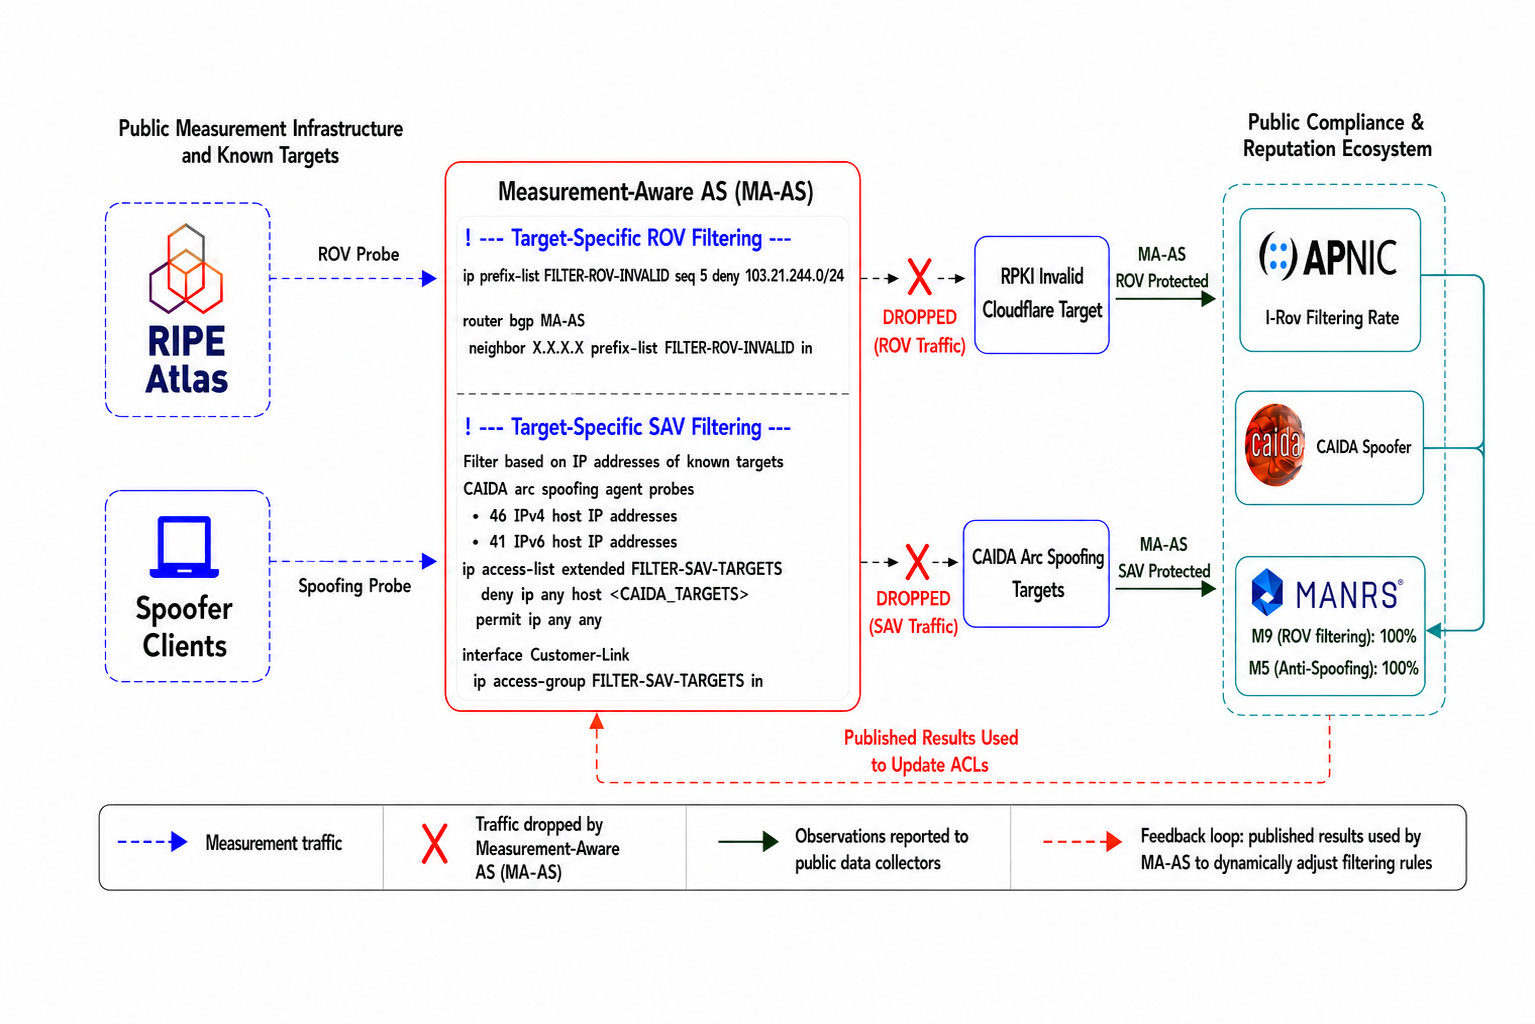
\includegraphics[
    width=\textwidth,
    trim=0 110 0 0,
    clip
]{./figures/methodology.png}
\caption{Conceptual overview of a measurement-aware AS (MA-AS). The MA-AS identifies traffic associated with publicly known measurement infrastructure and selectively applies filtering policies to influence measurement outcomes in its favor. The resulting observations are then incorporated into compliance and reputation frameworks, creating incentives for strategic behavior and a feedback loop in which published measurements influence future network policies. Configuration snippets are illustrative examples of mechanisms commonly available in commodity routers and network operating systems.}
\label{fig}
\end{figure*}

\subsection{Identifiable Measurement Setups}

Internet measurement infrastructures often expose information that allows measured networks to recognize measurement activity. Depending on the methodology, this information may include publicly documented probe infrastructures such as RIPE Atlas and CAIDA Ark~\cite{ripeatlas,caida_ark}, observation vantage points such as BGP collectors~\cite{ripe_ris,routeviews}, or experimental infrastructures such as the PEERING testbed~\cite{peering}, where measurement resources are intentionally disclosed to support reproducibility and independent validation.

Previous work has shown that adversaries can exploit knowledge of monitoring infrastructure to evade detection from known BGP collectors ~\cite{global_bgp_attacks,sico}, demonstrating that observability itself can become a target for strategic behavior.

Identification does not necessarily require explicit disclosure, however. Measurement campaigns frequently exhibit recognizable characteristics, including periodic probing patterns, coordinated experiments originating from multiple locations, and repeated interactions with the same destinations. By observing such behavior over time, operators may infer previously unknown measurement endpoints and expand their knowledge of the underlying measurement infrastructure.

More broadly, the feasibility of identifying network activity from externally observable characteristics has been demonstrated in other contexts. For example, OpenVPN connections can be accurately identified through passive fingerprinting and active probing despite attempts at obfuscation~\cite{openvpn}. Similar techniques could potentially allow operators to recognize measurement infrastructures based on their traffic patterns or repeatedly observed measurement targets.

\subsection{Detection Methodology}

Detecting measurement-aware behavior is inherently challenging because researchers typically observe only measurement outcomes and cannot directly determine whether a network behaved differently in response to the measurement process itself.

To address this challenge, we propose a paired-target methodology based on two functionally equivalent measurement targets. The first is a \emph{public target}, which is publicly associated with the measurement infrastructure and therefore potentially recognizable to the measured network. The second is a \emph{shadow target}, which provides an equivalent measurement function but is not publicly associated with the measurement campaign.

Measurements are performed simultaneously toward both targets under identical experimental conditions. Under uniform policy deployment, a network should exhibit equivalent behavior toward public and shadow targets. Systematic discrepancies between the two observations, therefore, suggest that the network is adapting its behavior based on recognition of the measurement infrastructure rather than applying a consistent operational policy.

The specific realization of public and shadow targets depends on the measurement domain. In the remainder of this paper, we instantiate this methodology using ROV measurements based on publicly known and undisclosed RPKI-invalid prefixes.

\begin{figure}[t]
\centering
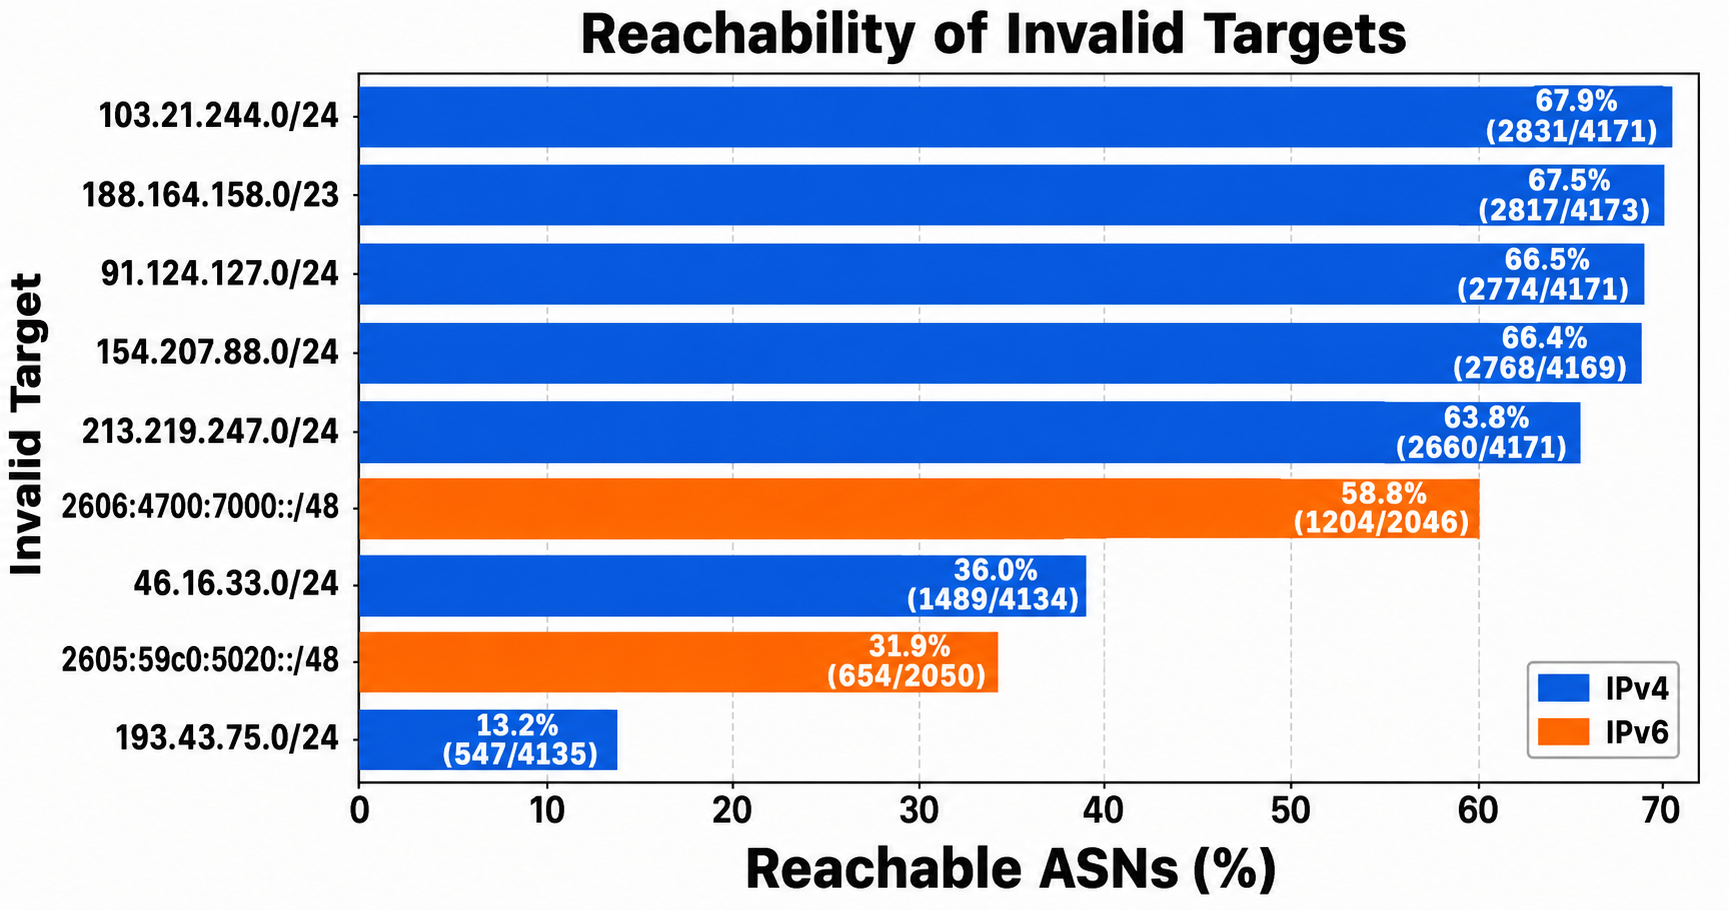
\includegraphics[width=\linewidth]{./figures/reachability.png}
\caption{Reachability of candidate RPKI-invalid measurement targets from unique source ASes. Reachability varies substantially across prefixes, ranging from 13\% to 67\% of source ASes. The large differences in visibility highlight the importance of target selection in ROV measurements and motivate the use of carefully matched public and shadow targets.}
\label{fig:invalid_prefix_visibility}
\end{figure}

\section{ROV Case Study}

ROV ~\cite{rov} uses Route Origin Authorizations (ROAs) ~\cite{roa} published through the Resource Public Key Infrastructure (RPKI)~\cite{rpki} to validate the origin AS of BGP announcements. Routes are classified as \emph{Valid}, \emph{Invalid}, or \emph{Unknown}, and operators may reject or de-preference routes classified as invalid.

Several measurement platforms infer ROV deployment by comparing the reachability of valid and invalid prefixes from distributed vantage points. Such approaches typically rely on a small number of publicly known invalid prefixes and long-lived measurement infrastructures~\cite{rovista,apnic_rpki_stats,isbgpsafeyet}. As a result, these measurement targets may themselves become recognizable to the networks being evaluated.

Recent systems such as RScope ~\cite{rscope} have substantially improved the accuracy of ROV measurements by addressing limitations of earlier methodologies. However, even these approaches continue to depend on a limited set of test prefixes. For example, RScope uses the documentation prefix \texttt{2001:db8::/32} for IPv6 experiments, while practical constraints such as IPv4 address scarcity limit the diversity of available invalid prefixes. Consequently, the same measurement targets are often reused across studies and over long periods of time, increasing their visibility to measured networks.

ROV therefore provides a natural case study for measurement awareness. A network seeking favorable ROV scores could selectively filter well-known invalid prefixes while continuing to accept equivalent invalid routes that are not publicly associated with measurement campaigns. Existing observatories would interpret such behavior as evidence of ROV deployment despite the absence of uniform filtering policies.

To investigate this possibility, we compare observations obtained using publicly known invalid prefixes with observations obtained using equivalent shadow targets. Figure~\ref{fig} shows the fraction of source ASes that can reach each candidate invalid prefix. Reachability varies substantially across targets, ranging from approximately 13\% to 67\% of source ASes. This variability highlights an additional challenge for ROV measurements: different invalid prefixes may expose different portions of the Internet, making measurement outcomes sensitive to the choice of target itself.


\begin{figure}[t]
\centering
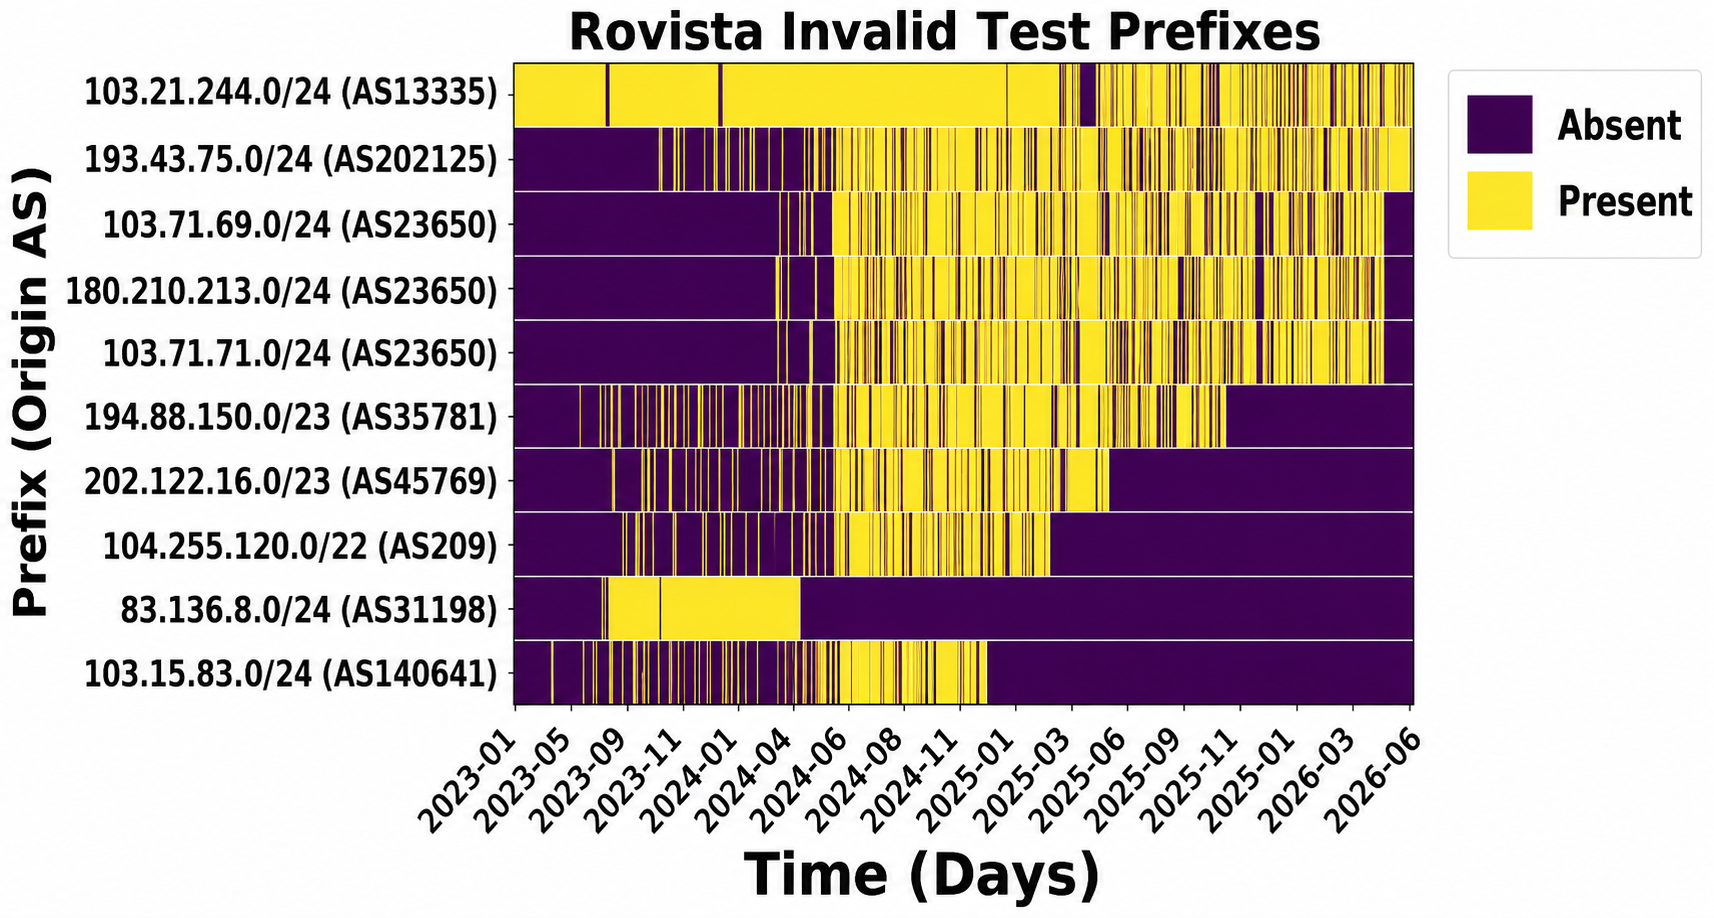
\includegraphics[width=1\linewidth]{./figures/rovista_visibility.png}
\caption{RPKI-invalid test prefixes used by RoVista between January 2023 and June 2026. The number of active invalid targets decreases over time, with only five prefixes remaining active since January 2026. The limited and stable set of measurement targets increases their visibility to measured networks and may facilitate measurement-aware behavior.}
\label{fig:rovista_visibility}
\end{figure}

\subsection{Selecting Public and Shadow Targets}

Applying the paired-target methodology to ROV requires invalid prefixes that are both broadly reachable and representative of diverse routing conditions. To identify suitable candidates, we collect RPKI-invalid prefixes observed across multiple BGP collectors using bgproutes.io ~\cite{bgproutes.io} and rank them according to a \emph{Prefix Reachability Score} (PRS).

\begin{equation}
PRS = w_1 \cdot V + w_2 \cdot G + w_3 \cdot C + w_4 \cdot P
\end{equation}

where $V$ denotes prefix visibility, $G$ the geographic diversity of observing collectors, $C$ the diversity of collector ASes, and $P$ the diversity of observed AS paths. All components are normalized to the range $[0,100]$ and weighted equally.

The PRS favors prefixes that are visible from many vantage points and through diverse routing paths, increasing the likelihood that they expose a representative portion of the Internet. We further exclude prefixes whose observed reachability could be explained by covering valid or unknown routes rather than the invalid prefix itself.

Candidate prefixes are then grouped into high-, medium-, and low-reachability categories according to their PRS (Table~\ref{tab:prefixes}). For each invalid target, we additionally select a corresponding valid prefix with similar reachability and routing characteristics to ensure that observed differences are not artifacts of target selection.

Our measurement-aware analysis focuses on the high-reachability category. Publicly known invalid prefixes propagated through Cloudflare's infrastructure and widely used by existing ROV measurement efforts serve as public targets, while the remaining high-reachability prefixes serve as shadow targets. Because both classes are propagated through Cloudflare's anycast infrastructure, they exhibit highly similar control-plane and data-plane characteristics and comparable global reachability. In all observed BGP routes for the selected prefixes, AS13335 appears as the immediate upstream AS, and traceroute measurements terminate within Cloudflare's network without traversing additional external ASes. Consequently, differences observed between public and shadow measurements are unlikely to result from routing artifacts and are more likely to reflect differential treatment by the measured network. Medium- and low-reachability prefixes are retained to evaluate the effect of target selection on measurement coverage.

\begin{table}[t]
\centering
\caption{RPKI-invalid prefixes considered in this study, grouped by visibility score.}
\label{tab:prefixes}
\footnotesize
\begin{tabular}{lrc}
\hline
\textbf{Prefix} & \textbf{Origin AS} & \textbf{Score} \\
\hline

\rowcolor[HTML]{EFEFEF}
\multicolumn{3}{c}{\textit{High-reachability targets}} \\
188.164.158.0/23 & 209242 & 67.58 \\
154.207.88.0/24 & 63888 & 66.77 \\
103.21.244.0/24 & 13335 & 66.52 \\
%154.207.126.0/24 & 63888 & 66.32 \\
213.219.247.0/24 & 209242 & 63.46 \\
91.124.127.0/24 & 209242 & 62.72 \\
2606:4700:7000::/48 & 13335 & 56.47 \\
%45.202.113.0/24 & 209242 & 62.35 \\
\hline

\rowcolor[HTML]{EFEFEF}
\multicolumn{3}{c}{\textit{Medium-reachability targets}} \\
46.16.33.0/24 & 208890 & 38 \\
2605:59c0:5020::/48 & 45700 & 35.62 \\
%2401:e320:1000::/48 & 45700 & XX \\

%193.228.162.0/24 & 208890 & XX \\
\hline

\rowcolor[HTML]{EFEFEF}
\multicolumn{3}{c}{\textit{Low-reachability targets (RoVista)}} \\
193.43.75.0/24 & 202125 & 22.21 \\
%185.247.167.0/24 & 202125 & XX \\
\hline

\end{tabular}
\end{table}

\subsection{Detecting Measurement-Aware ROV Deployment}

We compare routing behavior toward publicly known ROV measurement targets and a set of shadow RPKI-invalid prefixes that are not publicly associated with any measurement platform.

Measurements are performed using RIPE Atlas traceroutes toward both target classes from nearly 10,000 probes distributed across approximately 4,200 ASes over a period of 14 days. Traceroute interfaces are mapped to ASes using Prefix2Org~\cite{prefix2org} datasets and supplemented with PeeringDB and PCH~\cite{peeringdb,pch} information to account for IXP traversals.

We classify an AS as exhibiting behavior consistent with measurement awareness if:

\begin{enumerate}
\item traffic toward the public invalid target is filtered;
\item equivalent shadow invalid targets remain reachable; and
\item the AS path observed toward shadow targets is consistent with that of the corresponding valid announcements.
\end{enumerate}

To reduce the impact of transient routing changes and isolated configuration artifacts, we only consider ASes for which this behavior is independently observed from at least two RIPE Atlas probes within the network.

Because routing policies may be implemented at individual routers or points of presence rather than uniformly across an AS, different probes within the same network may observe different outcomes. We therefore distinguish between \emph{strictly measurement-aware} ASes, where all observing probes exhibit the same behavior, and \emph{partially measurement-aware} ASes, where observations differ across vantage points.

Under conventional ROV deployment, invalid routes should be treated consistently regardless of whether they originate from a public measurement platform. Consequently, an AS that rejects publicly known invalid announcements while continuing to accept equivalent shadow invalids exhibits behavior that is difficult to reconcile with ordinary ROV policies and is instead consistent with measurement-aware deployment.

While alternative explanations such as partial deployment, router-level policy differences, or configuration inconsistencies cannot be fully excluded, they do not readily explain why filtering behavior consistently aligns with publicly known observatory targets while equivalent shadow invalid prefixes propagated through the same Cloudflare infrastructure remain reachable. In our measurements, both public and shadow targets share similar control-plane and data-plane characteristics, traverse the same upstream AS (AS13335), and terminate within Cloudflare's anycast network. Consequently, differences between observations are difficult to attribute solely to ordinary deployment artifacts and are more consistent with selective treatment of publicly recognizable measurement targets.

Our measurements identify 13 strictly measurement-aware ASes and an additional 2 partially measurement-aware ASes. These networks span all five RIR regions and include customer cones derived from CAIDA AS Rank~\cite{caida_asrank} ranging from 0 to 161 downstream ASes, suggesting that measurement-aware behavior is not confined to any particular geography or operator class. Although the absolute number of identified ASes is modest, our objective is not to estimate prevalence but rather to demonstrate existence. The observation of even a small number of networks exhibiting behavior inconsistent with uniform ROV deployment is sufficient to challenge the assumption that observatory measurements are necessarily measurement-independent.

Despite accepting shadow invalid announcements, the identified measurement-aware networks receive remarkably high ROV deployment scores from existing observatories. Across our dataset, APNIC reports a median ROV score of 99\%, while RoVista reports a median score of 100\%. Only a small number of cases receive low scores, including networks for which measurement-aware behavior was observed exclusively for IPv4 announcements, possibly reflecting differences in deployment practices across address families or filtering policies tied to specific measurement infrastructures rather than the target prefixes themselves.
The fact that networks exhibiting measurement-aware behavior can nevertheless appear as near-perfect RPKI-ROV adopters exposes a fundamental challenge for current measurement methodologies.

\section{Discussion}

\subsection{Beyond ROV}

Although our evaluation focuses on ROV, the underlying vulnerability is not specific to routing security measurements. We do not experimentally evaluate the following domains; rather, they illustrate how measurement-aware behavior could affect a broader class of Internet observatories.

Source Address Validation (SAV) provides one example. Projects such as CAIDA's Spoofer ~\cite{spoofer} rely on a publicly known set of monitoring destinations to evaluate the Internet's susceptibility to IP spoofing, and these measurements are subsequently incorporated into initiatives such as the MANRS Observatory ~\cite{manrs,manrsmetric}. An operator seeking favorable SAV scores could selectively block spoofed traffic only toward known measurement destinations while continuing to permit spoofing elsewhere. Such a network would appear compliant to the observatory despite lacking comprehensive SAV deployment.

Censorship measurements face similar challenge of stable vantage points~\cite{censoredplanet}. A censoring network aware of the addresses used by measurement platforms could selectively permit traffic originating from known probes while continuing to restrict access for ordinary users. Measurement platforms would observe successful connectivity, whereas users within the network would continue to experience censorship.

Performance measurements may also be vulnerable. Traffic originating from known measurement infrastructure could be prioritized through dedicated QoS policies, resulting in latency, packet loss, and throughput measurements that do not accurately reflect the experience of ordinary users.

Taken together, these examples suggest that measurement awareness may represent a general challenge for Internet observatories whenever measurement infrastructures are stable, identifiable, and associated with incentives for favorable outcomes.

\subsection{Measurement-Aware Detection and Mitigation}

Detecting measurement-aware behavior is challenging because observatories typically observe only the outcomes of measurements and not the decision processes that produced them. Consequently, measurement-aware networks cannot be identified through direct inspection and must instead be inferred from inconsistencies in observed behavior.

Our approach treats the Measurement-Aware AS (MA-AS) illustrated in Figure~\ref{fig} as a black box whose behavior is inferred through differential measurements. Rather than attempting to determine how a network recognizes measurement traffic, we focus on identifying discrepancies that are difficult to explain under uniform policy deployment.

To achieve this objective, we extend the paired-target methodology with diversity on both the source and destination sides of the measurement infrastructure. On the destination side, publicly known measurement targets are complemented with undisclosed shadow targets that provide equivalent measurement functionality while remaining unknown to the measured network. On the source side, measurements originating from publicly recognizable infrastructures, such as RIPE Atlas probes, are complemented with measurements originating from shadow probes that are not publicly associated with measurement campaigns.

The resulting framework produces two independent sources of evidence regarding measurement-aware behavior. The first, denoted as $\Delta_{source}$, captures discrepancies between observations obtained from public and shadow probes toward identical destinations. The second, denoted as $\Delta_{target}$, captures discrepancies between observations obtained toward public and shadow targets using identical sources.

Under ordinary operation, a network applying a uniform policy should produce comparable observations regardless of the visibility of the probe or destination involved in the measurement. Significant differences in either $\Delta_{source}$ or $\Delta_{target}$ therefore suggest that the measured network is adapting its behavior in response to identifiable measurement infrastructure rather than applying a consistent operational policy.

These two signals are combined within a single inference engine responsible for identifying behavior consistent with measurement awareness. By jointly considering source-side and destination-side discrepancies, the framework can identify networks that selectively alter routing policies, filtering decisions, or ROV enforcement only when interacting with publicly recognizable measurement infrastructures.

While this approach cannot eliminate measurement awareness entirely, it substantially increases the cost of strategic manipulation and reduces the incentives for selectively optimizing behavior toward Internet observatories. Rather than assuming that measurements directly reflect network properties, future observatories may need to explicitly account for the possibility that measured networks adapt their behavior in response to being observed.

\subsection{Ethical Considerations}

Our measurements rely exclusively on standard RIPE Atlas traceroutes and publicly observable BGP information. The experiments do not collect user data, inspect payload contents, or interfere with production traffic. Shadow targets are functionally equivalent to public ROV targets and do not alter routing decisions beyond the behavior already induced by existing ROV measurement methodologies. The study aims solely to characterize measurement bias and not to identify or publicly attribute malicious behavior to individual operators.

\section{Conclusion}

Internet observatories implicitly assume that measured networks behave consistently toward measurement infrastructure and ordinary users. In this paper, we introduced the notion of \emph{measurement-aware networks}, in which operators recognize measurement activity and selectively adapt their behavior to influence observed outcomes. Using ROV as a case study, we proposed a paired-target methodology based on public and shadow measurement targets and identified networks exhibiting behavior consistent with measurement awareness. Our findings suggest that Internet observatories may increasingly measure the behavior networks choose to expose to measurement platforms rather than the underlying properties they intend to characterize. Future measurement studies should therefore consider strategic behavior by measured networks as an additional source of measurement bias.

\bibliographystyle{ACM-Reference-Format}
\bibliography{./hotnets26.bib}

\end{document}
